\documentclass[a4paper,12pt]{article}
\usepackage{amsmath}
\usepackage{amssymb}
\usepackage[utf8]{inputenc}
\usepackage[T1]{fontenc}
\usepackage{lmodern}
\usepackage{indentfirst}
\usepackage{geometry}
\usepackage{array}
\usepackage[pdftex]{color,graphicx}
\usepackage{subfigure}
\usepackage{afterpage}
\usepackage{setspace}
\usepackage{color}
\usepackage{wrapfig}
\usepackage{listings} 
\usepackage{datetime}
\usepackage{epstopdf}
\usepackage{hyperref}

\renewcommand{\onehalfspacing}{\setstretch{1.6}}

\geometry{tmargin=2.5cm,bmargin=2.5cm,lmargin=2.5cm,rmargin=2.5cm}
\setlength{\parindent}{1cm}
\setlength{\parskip}{0mm}

\newenvironment{lista}{
\begin{itemize}
  \setlength{\itemsep}{1pt}
  \setlength{\parskip}{0pt}
  \setlength{\parsep}{0pt}
}{\end{itemize}}

\newcommand{\linia}{\rule{\linewidth}{0.4mm}}

\definecolor{lbcolor}{rgb}{0.95,0.95,0.95}
\lstset{
  backgroundcolor=\color{lbcolor},
  tabsize=4,
  language=C++,
  captionpos=b,
  tabsize=3,
  frame=lines,
  numbers=left,
  numberstyle=\tiny,
  numbersep=5pt,
  breaklines=true,
  showstringspaces=false,
  basicstyle=\footnotesize,
  identifierstyle=\color{magenta},
  keywordstyle=\color[rgb]{0,0,1},
  commentstyle=\color{green},
  stringstyle=\color{red}
  }

\begin{document}

\noindent
\begin{tabular}{|c|p{11cm}|c|} \hline 
Michał Szczygieł & Aleksander Śmierciak & \ddmmyyyydate\today \tabularnewline
\hline 
\end{tabular}


\section*{Zadanie 4 - Trigramy - Wykrywanie języka}

Programem spełniającym polecenie zadania 4. jest taki, który przyjmując plik wejściowy uzyskany z wykonania programu z zadania 3. przeprowadzi dedukcję języka, w którym tekst z pliku został zapisany.
\\

Część programu odpowiedzialna za zrównoleglenie:

\begin{lstlisting}
      [...]
        #pragma omp parallel for num_threads(threadCount) \
                    shared(trigramsToCompare, result) \
                    firstprivate(files) schedule(dynamic)
            for (unsigned int i = 0; i < files->size(); ++i)
            {
                    result[files->at(i)] = compareTrigrams(
                        trigrams, trigramsToCompare[files->at(i)]);
            }
    [...]

double compareTrigrams(Histogram trigrams, Histogram trigramsToCompare)
{
    int maxCoverage = trigrams.size();
    int currentCoverage = 0;
    for (Histogram::iterator iti = trigrams.begin();
                             iti != trigrams.end();
                           ++iti)
    {
        for (Histogram::iterator itj = trigramsToCompare.begin();
                                 itj != trigramsToCompare.end();
                               ++itj)
        {
            if((*iti).first == (*itj).first)
            {
                currentCoverage++;
            }
        }
    }
    return (100 * currentCoverage) / (double) maxCoverage;
}
\end{lstlisting}

Wcześniejsza implementacja:

\begin{lstlisting}
	#pragma omp parallel num_threads(threadCount)
	{
		std::string threeLetters;
		unsigned int endPosition = portion * (omp_get_thread_num() + 1);

		if (endPosition > contents.size())
		{
			endPosition = contents.size();
		}

		#pragma for default(none) shared(contents, trigram) firstprivate(portion) private(threeLetters)
		for (int i = portion * omp_get_thread_num();
				i != portion * (omp_get_thread_num() + 1); i += 3)
		{
			threeLetters = std::string(contents.substr(i, 3));
			trigram[threeLetters]++;
		}
	}
\end{lstlisting}


\section*{Przebieg}
Obliczenia zostały wykonane na serwerze CUDA. \\



Poniżej wykresy przedstawiający rezultat przeprowadzonych operacji na wątkach.
\\
\begin{center}
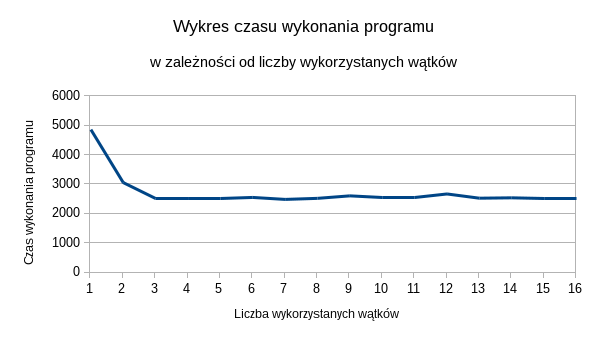
\includegraphics[width=0.7\textwidth]{data/wykonanie.png}
\end{center}


\begin{center}
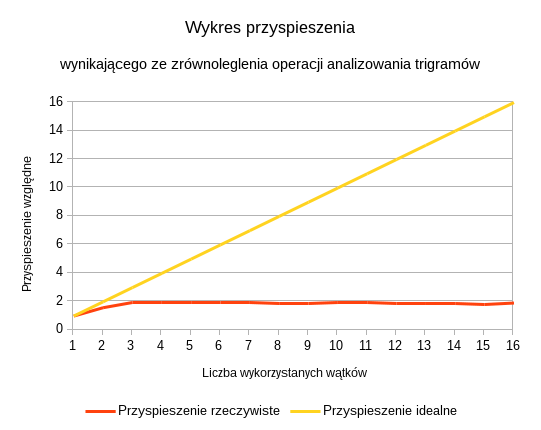
\includegraphics[width=0.7\textwidth]{data/przyspieszenie.png}
\end{center}

\end{document}